\newpage
\chapter{Elektrony a vakuum}
Před samotným započetím sestavování experimentu bylo nejdříve nutné pochopit podstatu chování elektronů při sníženém tlaku. Teprve pak bylo možné fokusovací a urychlovací aparaturu sestrojit. Tato kapitola se tedy věnuje základní charakteristice elektronů a jejich pohybu v prostředí se sníženým tlakem.

\section{Elektron}
Elektron je elementární částice se záporným elektrickým nábojem, která tvoří obal atomového jádra. V rámci Standardního modelu řadíme elektron do první generace skupiny leptonů. Jeho klidová hmotnost je $m_{0}=0,510~\mathrm{MeV}/c$ \cite{01Elektron} a spin 1/2. Poloviční spin jej řadí mezi fermiony, takže podléhá Pauliho vylučovacímu principu.

Elektrony jsou nositeli náboje při vedení elektrického proudu a také tvoří $\beta^{-}$ záření.

Elektron byl poprvé popsán v roce 1897 britským fyzikem J. J. Thomsonem, který takto vysvětlil podstatu katodového záření. Toto záření ale bylo pozorováno už v polovině 19. století W. Crooksem a několika dalšími fyziky. Experiment byl tvořen skleněnou (katodovou) trubicí s elektrodami naplněnou vzduchem nebo jiným plynem. Pokud byl v trubici dostatečně nízký tlak (asi tisícina atmosférického tlaku) a na elektrody bylo přivedeno vysoké napětí (více než 1000 V), objevilo se v trubici záření. Při dalším snižování tlaku bylo možné záření pozorovat i na stěně trubice, která se nacházela naproti katodě. Toto záření bylo označeno jako katodové záření a později Thomsonem popsáno jako proud elektronů.

\section{Katodové záření}
Katodové záření vzniká ve skleněné trubici se dvěma elektrodami. V této katodové trubici, ve které se nachází zředěný plyn, dochází při přivedení napětí na elektrody a postupném snižování tlaku k různým efektům spojeným s pohybem částic. Při tlaku zhruba 5 300 Pa se v trubici objevuje úzký sloupec vlnící se červený sloupec, který vychází z anody a končí těsně před katodou. Při dalším ředění plynu se sloupec rozšiřuje a zkracuje a vzniká tzv. anodový sloupec, který je od katody oddělen tmavým tzv. Faradayovým prostorem. Na katodě přitom vzniká doutnavé katodové světlo. Budeme-li se zřeďováním pokračovat, bude anodový sloupec v trubici blednout a stávat se vrstevnatým. Katodové světlo pak pokrývá celou katodu. Pokud dosáhneme hranici tlaku zhruba 2,67 Pa, molekuly plynu již v trubici nepřekážejí pohybu elektronů a iontů, které se pak šíří prostorem přímočaře a s velkou rychlostí. Veškeré světelné úkazy pak v trubici mizí a dochází pouze k fluorescenci stěn trubice. Fluorescence je vyvolána proudem elektronů letících z katody, jinak nazývaných katodové záření. Jednotlivé fáze zřeďování plynu jsou na Obr. \ref{01katody}

\begin{figure}[htbp!]
\centering
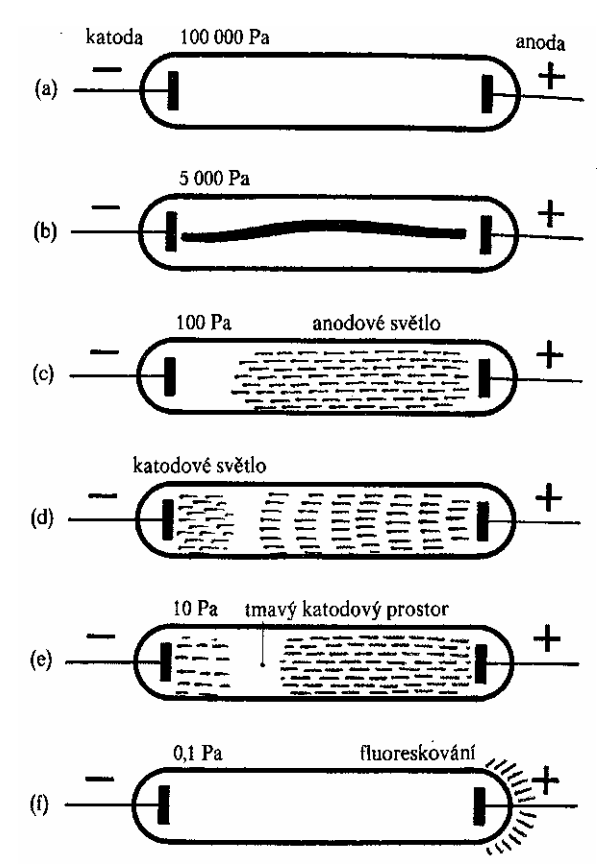
\includegraphics[width = 170 pt]{Figure/01/katody.png}
\caption[Efekty v katodové trubici při snižování tlaku.]{Efekty v katodové trubici při snižování tlaku. Převzato z~\cite{Plyny}}
\label{01katody}
\end{figure}

Jelikož bylo toto záření v průběhu let hojně zkoumáno, byly také pozorovány tyto jeho specifické vlastnosti:
\begin{itemize}
\item nepůsobí-li na něj vnější elektrické nebo magnetické pole, šíří se rovnoměrně přímočaře,
\item je vychylováno elektrickým a magnetickým polem,
\item interaguje s látkou, způsobuje zahřátí, světélkování a chemické procesy,
\item proniká tenkými vrstvami a rozptyluje se,
\item při dopadu na kovy s vysokou relativní atomovou hmotností vyvolává RTG záření,
\item má mechanické účinky (pokus s roztočením Crooksova mlýnku).
\end{itemize}

Elektronový svazek se využívá v obrazovkách osciloskopu a dříve také ve starých televizích a monitorech. V těchto zařízeních je elektronový svazek vychylován elektrickým nebo magnetickým polem. Na stejném principu funguje i náš experiment.

\section{Elektrický proud ve vakuu}
Vakuem obecně elektrický proud neprochází, jelikož neobsahuje nabité částice. Aby mohl proud vakuem procházet, je nutné uvolnit nositele náboje na elektrodách.

Jak už bylo zmíněno výše, tok elektronů ve vakuu má velké praktické využití a je důležitý i pro náš experiment. Jeho široké využití je založeno na těchto vlastnostech elektronů:

\begin{itemize}
\item mají nepatrnou hmotnost, proto mají ze všech částic největší měrný náboj, takže i ve slabých elektrických nebo magnetických polích získávají velkou rychlost na poměrně krátké dráze,
\item přenos náboje u nich prakticky není spojen s přenosem látky,
\item lze je snadno získat mnoha způsoby uvolňováním z kovů.
\end{itemize}

Uvolňování elektronů z kovů probíhá zahřátím vodiče na vysokou teplotu, čímž získají některé elektrony, které se za normálních okolností ve vodiči neuspořádaně pohybují, dostatečnou rychlost, aby překonaly vnitřní přitažlivé síly a vylétly z vodiče ven. Tomuto jevu se říká termoemise. Při termoemisi se původně neutrální vodič stává kladně nabitým, což způsobuje následné přitahování elektronů zpět na povrch vodiče, čímž vzniká tzv. elektronový mrak. 

%princip změny polohy?
%
%\begin{figure}[htbp!]
%\centering
%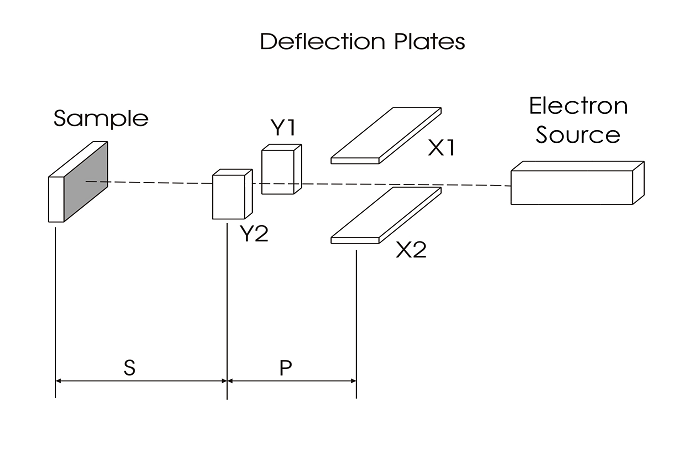
\includegraphics[width = 170 pt]{Figure/04/schema2.png}
%\caption{. Převzato z~\cite{Manual}}
%\label{04schema2}
%\end{figure}

